
\documentclass[pdftex, a4paper]{scrartcl}	% twoside is default option for scrbook

\usepackage{amsmath}
\usepackage{graphics} % for improved inclusion of graphics


\title{The transient function - a short overview} 
\author{Clemens Kreutz}
\date{}
\begin{document}
\maketitle
\section{Abstract}
The transient function $f(t)$ is a powerful tool for describing the dynamics of transient systems.
It can be applied to experimental data as well as to approximate the dynamics of ODE models.
The parameters of the function provide an intuitive interpretation in terms of time-scales and amplitudes of
sustained and transient responses.


\section{The 6-parameter transient function}
The dynamics of transient systems can be approximated by fitting a five parameter transient function
\begin{equation}  \label{eq:f5para}
	f(t) =  A_{\text{sus}} \left( 1-  e^{-\frac t {\tau_1}}\right)   + A_{\text{trans}} \left(1-e^{-\frac t {\tau_1'}}\right) e^{-\frac t {\tau_2}} + p_0 
\end{equation}
to the time courses.
To prevent overfitting, only two time scale parameters are allowed, i.e.~$\tau_1\equiv\tau_1'$.
This model has five independent parameters 
\begin{equation}
	\vec \theta := \{A_\text{sus},A_\text{trans},\tau_1, \tau_2, p_0\}\:\:.
\end{equation}
The first term in ($\ref{eq:f5para}$) represents a sustained response with amplitude $A_\text{sus}$ and time-constant $\tau_1$ which corresponds to the duration it takes until the sustained part of the response.
The second term accounts for transient up- or down-regulation with amplitude $A_\text{trans}$.
To prevent overfitting (which is recommended if a limited amount of data is available),
the same time constant $\tau_1$ for induction of the transient response is assumed as for the sustained response. 
The transient response relaxes with second time scale $\tau_2$ towards zero.
The last parameter $p_0$ is the offset which is specified during fitting primarily by the measurement at $t=0$.
If the data is preprocessed, e.g.~by subtracting the minimal value, the offset parameter $p_0$ might be omitted.

The five-parameter function describes immediate responses at starting at time-point zero and should only applied, 
if an immediate response after stimulation is expected.
If in this case the data contains measurements within the (long) constant interval before stimulation,
it might be required to pre-process the data properly, i.e.~ remove the time interval before stimulation or shift
measurements before stimulation to $t=0$.

The five-parameter transient function was used in \cite{Lucarelli} for analyzing the transcription of TGF$\beta$ target genes.
In this application, the analyses were performed for pairs of time-courses for treated and untreated cells.
A corresponding setting is provided as \emph{Example1}.
In this illustration example, specific parameters for each compound/experiment are created by using D2D's ``random effects'' option. This enables usage of a column in the data table for specifying which data sets are fitted with common or distinct parameters.

In order to 

\section{Up- and downwards response}
The five-parameter transient function ($\ref{eq:5para}$) allows positive and negative amplitudes.
In many application settings, however, it might be a reasonable assumption, that the sustained and transient part of the response have the same direction, i.e.~are both either upwards or both downwards.
This also reduced the amount of overfitting and often yields much more realistic outcomes.
It can be achieved by restricting both amplitudes to positive numbers and introducing a sign-constant.
If such a model is fitted, two optimization runs are required for both signs and the better fit is selected.
This procedure is implemented in D2D in \texttt{arFitTransient.m}.

The transient function is non-linear often exhibits local maxima. 
Therefore, multi-start optimization might be necessary to find the global optimum, i.e.~the global best fit.
In D2D, this is implemented in \texttt{arFitLHS.m} which generates random initial guesses and the calles \texttt{arFits.m} to perform several fits for the random initial guesses.
If the transient function is implemented with discrete sign constants, \texttt{arFits} has to call \texttt{arFitTransient} instead of \texttt{arFit}. 
Therefore, the standard-function in \texttt{arFramework3/Advanced/arFits.m} has to be replaced by \texttt{arFramework3/Examples/ToyModels/TransientFunction/TransientFunction\_library/arFits.m} by properly setting Matlab's search path.


\section{Error parameter}
For fitting, a maximum likelihood approach is used, i.e. an objective function
\begin{equation} \label{eq:LL}
	F(\vec \theta) := -2 \log L(y|\vec\theta) = -2 \sum_i \log \left( \frac 1 {\sqrt{2\pi}\sigma} \right) + \sum_i \left(  \frac{y_i - f_i}{\sigma_i} \right)^2
	\end{equation}
	is minmized for estimation the parameters:
	\begin{equation}
		\hat \theta = \arg  \min_{\vec \theta} F(\vec\theta)
	\end{equation}
	Equation $\ref{eq:LL}$ is obtained if the likelihood for Gaussian errors is utilized. 
	$\sigma$ corresponds to the standard deviation of Gaussion noise.
	It is used as an unknown parameter and corresponds and can be interpreted as an approximation error.

\subsection{Retarded transient dynamics}
\begin{figure}[!t]
\begin{center}
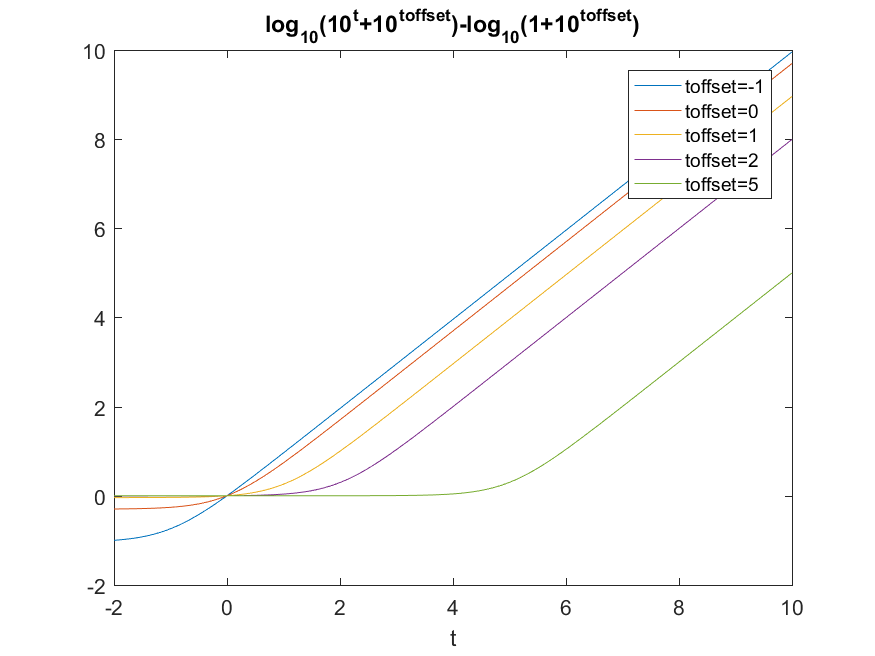
\includegraphics{TimeOffset_TransientFunction.png}
\end{center}
\caption{Transformation of the time axis to account for retarded transient dynamics. \label{fig:retarded}}
\end{figure} 

Depending on the application example, the transient dynamics does not start at $t=0$ but is delayed.
This setting is accounted by a nonlinear transformation of the time-axis with a single parameter $t_\text{shift}$.
The transformation is illustrated in Figure xxx.


\section{Parameter bounds}
If a small number of data points is available, it is essential to prevent overfitting.
This can be achieved by 
\begin{itemize}
\item 	specifying bound for the parameters for restriction to reasonable ranges
\item  only two time scale parameters are allowed, i.e.$\tau_1\equiv\tau_3$
\end{itemize}

%\begin{center}
\begin{table}
%\begin{minipage}[c]{1.1\linewidth}
\begin{tiny}
\begin{tabular}{|c|l|l|l|l|}
\hline
Symbol & Description & lower bound & upper bound & default initial guess  \\ \hline
$\tau_1$ 	& Time-scale/duration of the response &  $\min_i (t_{i+1} - t_{i})/2$   	&  $2(t_{\max}-t_{\min})$  			& $0.5 \text{lb} + 0.5 \text{ub}$\\
$\tau_2$ 	& duration slower transient decrease   &  $\min_i (t_{i+1} - t_{i})/2$   	&  $2(t_{\max}-t_{\min})$  			& $0.5 \text{lb} + 0.5 \text{ub}$\\ \hline
$A_\text{sus}$ & Amplitude of the sustained response & -$2 (\max(y) - \min(y))$	&  $2 (\max(y) - \min(y))$ 				& $0.1 \text{lb} + 0.9 \text{ub}$\\ 
$A_\text{trans}$ & Amplitude transient decrease & -$2 (\max(y) - \min(y))$				&  $2 (\max(y) - \min(y))$ 			   &  $0.1 \text{lb} + 0.9 \text{ub}$\\ \hline
$p_0$ 	& data offset 												& $\min(y)$  										&  $\max(y)$ 										&  $0.5 \text{lb} + 0.5 \text{ub}$ \\
$\sigma$ 	& approximation error 							& $(\max(y) - \min(y))/10 000$ 		&  $(\max(y) - \min(y))$ 					&  $\text{SD}(y)$	\\ \hline
$t_\text{shift}$ & response time									& -2 														& 5 															&  -1 \\ \hline
\end{tabular}
\end{tiny}
%\end{minipage}
\caption{Suggested default values and parameter bounds. \label{tab:bounds}}
\end{table}
%\end{center}

\end{document}

